\chapter{\IfLanguageName{dutch}{Stand van zaken}{State of the art}}%
\label{ch:stand-van-zaken}

% Tip: Begin elk hoofdstuk met een paragraaf inleiding die beschrijft hoe
% dit hoofdstuk past binnen het geheel van de bachelorproef. Geef in het
% bijzonder aan wat de link is met het vorige en volgende hoofdstuk.

% Pas na deze inleidende paragraaf komt de eerste sectiehoofding.

\begin{comment}

Dit hoofdstuk bevat je literatuurstudie. De inhoud gaat verder op de inleiding, maar zal het onderwerp van de bachelorproef *diepgaand* uitspitten. De bedoeling is dat de lezer na lezing van dit hoofdstuk helemaal op de hoogte is van de huidige stand van zaken (state-of-the-art) in het onderzoeksdomein. Iemand die niet vertrouwd is met het onderwerp, weet nu voldoende om de rest van het verhaal te kunnen volgen, zonder dat die er nog andere informatie moet over opzoeken \autocite{Pollefliet2011}.

Je verwijst bij elke bewering die je doet, vakterm die je introduceert, enz.\ naar je bronnen. In \LaTeX{} kan dat met het commando \texttt{$\backslash${textcite\{\}}} of \texttt{$\backslash${autocite\{\}}}. Als argument van het commando geef je de ``sleutel'' van een ``record'' in een bibliografische databank in het Bib\LaTeX{}-formaat (een tekstbestand). Als je expliciet naar de auteur verwijst in de zin, gebruik je \texttt{$\backslash${}textcite\{\}}.
Soms wil je de auteur niet expliciet vernoemen, dan gebruik je \texttt{$\backslash${}autocite\{\}}. In de volgende paragraaf een voorbeeld van elk.

\textcite{Knuth1998} schreef een van de standaardwerken over sorteer- en zoekalgoritmen. Experten zijn het erover eens dat cloud computing een interessante opportuniteit vormen, zowel voor gebruikers als voor dienstverleners op vlak van informatietechnologie~\autocite{Creeger2009}.

\end{comment}


\section{Wat is Microsoft administration?}


\section{Azure Active Directory Graph}

\subsection{Wat is Active Directory?}

\ac{AD} is een centrale en gemeenschappelijke opslagplaats voor informatie geïntroduceerd door Microsoft \autocite{Allen2003}. De eerste versie van \ac{AD} is gemaakt voor de Windows 2000 server-editie. Deze opslagplaats bevat allerlei informatie binnen een netwerk, zoals gebruikers, groepen, computers, applicaties, bestanden en printers. Deze informatie kan worden opgevraagd en beheerd.

\subsection{Wat is Azure Active Directory?}

Azure \ac{AD} is een modernere aanpak van Active Directory binnen de cloud dat ontstaan is in 2008 \autocite{Chappell2008}. Azure \ac{AD} is een gecentraliseerd beheerplatform van Microsoft voor gebruikers en apparaten in netwerken die een verbinding hebben met de Azure-clouddienst \autocite{Mayank2019}. Middelen, waaronder gebruikers en apparaten, kunnen vanuit Azure \ac{AD} beheerd worden met bijhorende netwerkauthenticatie. Het dient als een centraal punt van informatie, waarbij details over alle middelen in het netwerk worden opgeslagen.

\subsection{Wat is Azure Active Directory met PowerShell?} 

Azure \ac{AD} PowerShell voor Graph, kortweg Azure \ac{AD} PowerShell, is een module binnen PowerShell dat gebruikt kan worden om Azure \ac{AD} te beheren \autocite{Microsoft2023}. PowerShell is een oplossing van Microsoft voor taakautomatisering via een \ac{CLI} \autocite{Microsoft2022}. \\

PowerShell staat gekend voor zijn breed scala aan informatie dat het kan verkrijgen. Dit breed scala gaat van systemen, servers, randapparatuur, mobiele apparaten tot gegevensgestuurde toepassingen zoals Active Directory \autocite{Hosmer2019}. Vandaag de dag ondersteunt PowerShell meer dan 11.350 unieke modules en scripts via de PowerShell Gallary, waaronder de Azure \ac{AD} PowerShell module \autocite{Microsoft2023a}. \\

Door het gebruik van Azure \ac{AD} in combinatie met PowerShell, wordt er gebruikgemaakt van het beste van de twee werelden. Een gecentraliseerd beheerplatform automatisch doen werken brengt bijkomende voordelen voor de maker. Uit onderzoek van \textcite{Breton2003} zijn enkele voordelen van automatisatie minder stress, tijdbesparing en een lagere kans op menselijke fouten.

\subsection{Wat is Azure Active Directory Graph?}

De communicatie tussen Azure AD en de Azure AD PowerShell module gebeurd via een API. Deze API is een REST API dat Graph wordt genoemd. De naam “Graph” (graaf in het Nederlands) staat voor de verbindingen tussen de entiteiten dat het ondersteunt, een principe dat voorkomt in de wiskunde (zie figuur \ref{mga}) \autocite{Kokkarinen2022}. Microsoft gebruikt deze wiskundige graaf als interpretatie van Graph (zie figuur \ref{gms}). 

\begin{figure}
    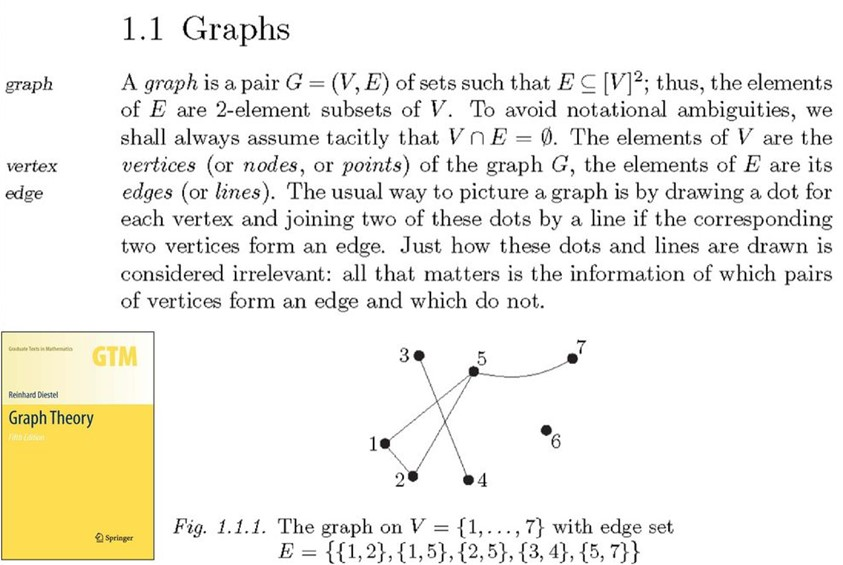
\includegraphics[width=\textwidth]{MathGraphExample.jpg}
    \caption[Voorbeeld wiskundige graaf]{Voorbeeld van een graaf in de wiskunde uit het boek Graph Theory van \textcite{Diestel2010}.}
    \label{mga}
\end{figure}

\begin{figure}
    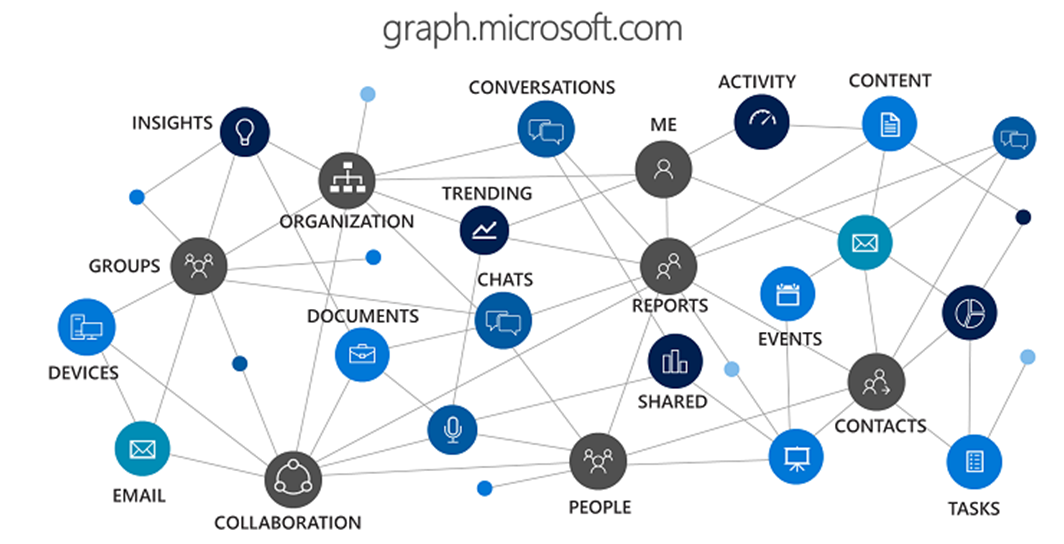
\includegraphics[width=\textwidth]{GraphMicrosoft.png}
    \caption[Voorbeeld Microsoft graaf]{Figuurlijke voorstelling van Graph binnen \textcite{Microsoft2017}.}
    \label{gms}
\end{figure}

\subsection{Toepassingen van Azure AD via PowerShell en Graph} 


\section{Microsoft Graph}

\lipsum[10-12]




